\documentclass[12pt]{article}

\usepackage{fontspec}
\setmainfont{TeX Gyre Termes}

\usepackage{geometry}
\geometry{margin=1in}

\usepackage{tikz}
\usetikzlibrary{arrows.meta, positioning}

\usepackage{hyperref}

\title{USRP X410 Interfaces and Control Workflow}
\date{}

\begin{document}

\maketitle

\section{Overview}

The USRP X410 supports two main host interaction workflows:

\begin{itemize}
\item UHD streaming via Ethernet (10/100 GbE)
\item NI-USRP + LabVIEW FPGA via PCIe
\end{itemize}

Additionally, the device includes a dedicated 1 GbE management port used
for configuration and control.

\section{Network and PCIe Interfaces}

The X410 provides the following external interfaces:

\begin{itemize}
\item 2 $\times$ QSFP28 ports supporting 10 GbE / 100 GbE
\item 1 $\times$ RJ45 port for 1 GbE management
\item iPass+ zHD PCIe interface for FPGA toolflow
\end{itemize}

\section{Control and Data Flow Architecture}

Figure~\ref{fig:x410_arch} illustrates the typical connection architecture.

\begin{figure}[h]
\centering

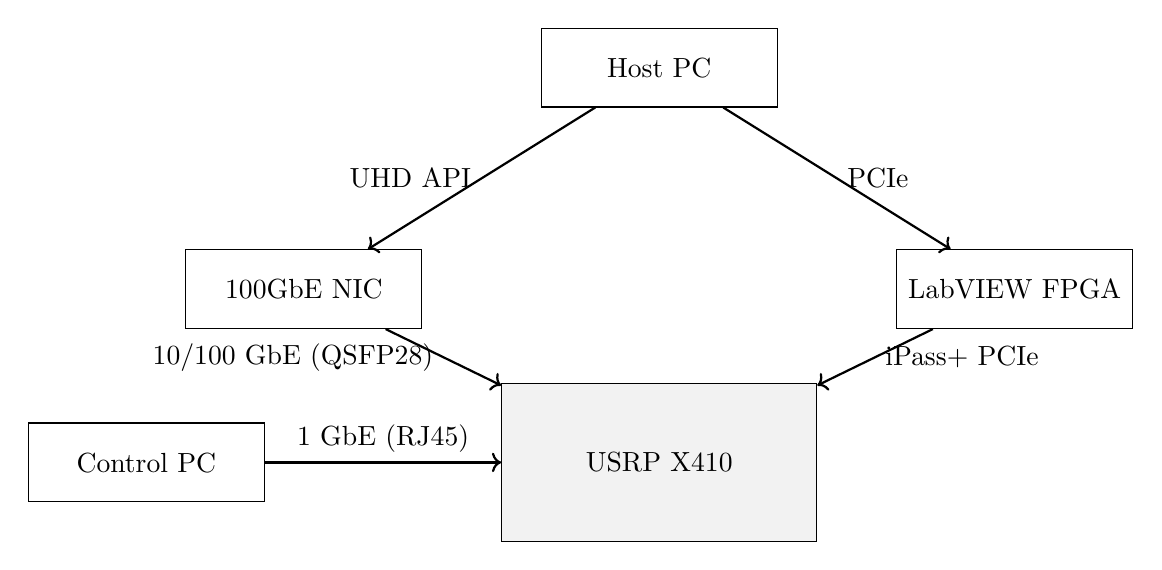
\begin{tikzpicture}[
node distance=2.5cm,
block/.style={draw, rectangle, minimum width=3cm, minimum height=1cm},
device/.style={draw, rectangle, minimum width=4cm, minimum height=2cm, fill=gray!10},
arrow/.style={->, thick}
]

% Host PC
\node[block] (host) {Host PC};

% NIC
\node[block, below left=1.8cm and 1.5cm of host] (nic) {100GbE NIC};

% LabVIEW
\node[block, below right=1.8cm and 1.5cm of host] (labview) {LabVIEW FPGA};

% X410
\node[device, below=3.5cm of host] (x410) {USRP X410};

% Management PC
\node[block, left=3cm of x410] (mgmt) {Control PC};

% Connections
\draw[arrow] (host) -- node[right]{PCIe} (labview);
\draw[arrow] (labview) -- node[right]{iPass+ PCIe} (x410);

\draw[arrow] (host) -- node[left]{UHD API} (nic);
\draw[arrow] (nic) -- node[left]{10/100 GbE (QSFP28)} (x410);

\draw[arrow] (mgmt) -- node[above]{1 GbE (RJ45)} (x410);

\end{tikzpicture}

\caption{USRP X410 host connectivity architecture}
\label{fig:x410_arch}

\end{figure}

\section{Ethernet Interface Details}

The two high-speed Ethernet ports are QSFP28 connectors supporting:

\begin{itemize}
\item 10 GbE
\item 100 GbE
\item Aurora links (depending on FPGA configuration)
\end{itemize}

Common cable types include:

\begin{itemize}
\item QSFP28 DAC (Direct Attach Cable)
\item QSFP28 AOC (Active Optical Cable)
\item Optical modules such as 100GBASE-SR4 or 100GBASE-LR4
\end{itemize}

\section{Management Port}

The RJ45 port provides a 1 GbE management interface used for:

\begin{itemize}
\item Device configuration
\item Control communication
\item System monitoring
\end{itemize}

This port does not carry high-rate IQ streaming data.

\section{LabVIEW and C++ Integration}

A C++ program can be compiled into a DLL and called from LabVIEW using the
\textit{Call Library Function Node}. Exported functions should follow a C ABI:

\begin{verbatim}
extern "C" __declspec(dllexport)
\end{verbatim}

Basic data types such as integers, doubles, and buffers should be used
to ensure compatibility.

However, when using the PCIe workflow with LabVIEW FPGA, NI's native
APIs are typically preferred instead of wrapping UHD functions.

\section{References}

\begin{itemize}
\item \href{https://www.ni.com/docs/en-BS/bundle/usrp-x410-getting-started/page/getting-started.html}{NI USRP X410 Getting Started Guide}
\item \href{https://www.ni.com/docs/en-DM/bundle/ettus-usrp-x410-specs/page/specs.html}{USRP X410 Specifications}
\item \href{https://files.ettus.com/manual/page_usrp_x4xx.html}{Ettus USRP X4xx Manual}
\end{itemize}

\end{document}